\documentclass[12pt,letterpaper]{article}

\def\myauthor{John~O.~Woods}
\def\mytitle{jow-vita}
\def\myemail{john.o.woods@gmail.com}
\def\myweb{johnowoods}
\def\myphone{703-801-2625}
\def\mykeywords{
  john woods,
  john o woods,
  john oates woods,
  resume, 
  curriculum, 
  vita, 
  curriculum vita, 
  cv, 
  john, 
  woods, 
  jow
}

\setlength\parindent{0pt}

\newenvironment{itemize*}%
{\begin{itemize}%
  \setlength{\itemsep}{0pt}}%
{\end{itemize}}

\usepackage{graphicx}
\usepackage{wrapfig}
\usepackage{amsmath}
\usepackage{url}
\usepackage{fancyhdr}
\usepackage{lastpage}
%\usepackage{ocgtools}
\usepackage{enumitem}
\setlist{nolistsep,leftmargin=0.15in}
\usepackage[log-declarations=false]{xparse}
%\usepackage{mathdesign}
%\usepackage[no-math]{fontspec}
\usepackage{microtype}
\usepackage[margin=1.125in,top=1.375in,right=1in,left=2in]{geometry}
\usepackage[strict]{changepage}
\usepackage[
  ocgcolorlinks,
  urlcolor={[rgb]{0,0,0.54}},
  unicode,
  plainpages=false,
  pdfpagelabels,
  pdftitle={\mytitle},
  pdfauthor={\myauthor},
  pdfkeywords={\mykeywords}
]{hyperref}
\usepackage{relsize}

% fix ocgcolor link breaking; thanks due to Benjamin Lerner (http://goo.gl/VZKR7M)
\makeatletter
\AtBeginDocument{%
  \newlength{\temp@x}%
  \newlength{\temp@y}%
  \newlength{\temp@w}%
  \newlength{\temp@h}%
  \def\my@coords#1#2#3#4{%
    \setlength{\temp@x}{#1}%
    \setlength{\temp@y}{#2}%
    \setlength{\temp@w}{#3}%
    \setlength{\temp@h}{#4}%
    \adjustlengths{}%
    \my@pdfliteral{\strip@pt\temp@x\space\strip@pt\temp@y\space\strip@pt\temp@w\space\strip@pt\temp@h\space re}}%
  \ifpdf
    \typeout{In PDF mode}%
    \def\my@pdfliteral#1{\pdfliteral page{#1}}% I don't know why % this command...
    \def\adjustlengths{}%
  \fi
  \ifxetex
    \def\my@pdfliteral #1{\special{pdf: literal direct #1}}% isn't equivalent to this one
    \def\adjustlengths{\setlength{\temp@h}{-\temp@h}\addtolength{\temp@y}{1in}\addtolength{\temp@x}{-1in}}%
  \fi%
  \def\Hy@colorlink#1{%
    \begingroup
      \ifHy@ocgcolorlinks
        \def\Hy@ocgcolor{#1}%
        \my@pdfliteral{q}%
        \my@pdfliteral{7 Tr}% Set text mode to clipping-only
      \else
        \HyColor@UseColor#1%
      \fi
  }%
  \def\Hy@endcolorlink{%
    \ifHy@ocgcolorlinks%
      \my@pdfliteral{/OC/OCPrint BDC}%
      \my@coords{0pt}{0pt}{\pdfpagewidth}{\pdfpageheight}%
      \my@pdfliteral{F}% Fill clipping path (the url's text) with current color
      \my@pdfliteral{EMC/OC/OCView BDC}%
      \begingroup%
        \expandafter\HyColor@UseColor\Hy@ocgcolor%
        \my@coords{0pt}{0pt}{\pdfpagewidth}{\pdfpageheight}%
        \my@pdfliteral{F}% Fill clipping path (the url's text) with \Hy@ocgcolor
      \endgroup%
      \my@pdfliteral{EMC}%
      \my@pdfliteral{0 Tr}% Reset text to normal mode
      \my@pdfliteral{Q}%
    \fi
    \endgroup
  }%
}
\makeatother
% end fixes


\newcommand{\Cpp}{\textsc{c}\nolinebreak[4]\hspace{-.05em}\raisebox{.4ex}{\relsize{-3}{\textbf{++}}}}
\newcommand{\Magickpp}{Magick\nolinebreak[4]\hspace{-.05em}\raisebox{.4ex}{\relsize{-3}{\textbf{++}}}}
\newcommand{\Star}{\textsc{Star-CCM\ensuremath{+}}}

\newcommand{\mhead}[1]{\leavevmode\marginpar{\sffamily\footnotesize #1}}
%\newcommand{\rdate}[1]{{\addfontfeature{Numbers=OldStyle} \hfill #1}}
%\renewcommand{\date}[1]{{\addfontfeature{Numbers=OldStyle} #1}}
\newcommand{\rdate}[1]{{\hfill #1}}
\renewcommand{\date}[1]{{#1}}
\renewcommand{\labelitemi}{-} 

%\setmainfont[
%  Ligatures={TeX,Common},
%  BoldFont={AGaramondPro-Semibold},
%]{Adobe Garamond Pro}
%\setsansfont[
%  Ligatures={TeX,Common},
%  Letters=SmallCaps,
%  Color=660000,
%]{Adobe Garamond Pro}
%\setmonofont[Scale=0.85]{FontAwesome}

%\makeatletter % fix for \hrulefill w/ mathdesign package
%\def\hrulefill{\leavevmode\leaders \hrule height \rulethickness \hfill\kern\z@}
%\makeatletter

\begin{document}\flushbottom
\pagestyle{fancy} \setlength\headwidth{6.5in}
\rhead{\textsc{Dr.~John~O.~Woods --- curriculum vitae --- \thepage{} of \pageref*{LastPage}}} \cfoot{}
\thispagestyle{empty}
\begin{adjustwidth}{-1in}{}
{\Huge
  {\textsc{%
    {%\addfontfeature{Style=TitlingCaps}
    J}\kern-1.0ptohn 
    {%\addfontfeature{Style=TitlingCaps}
    O}\kern-2pt.~%
    {%\addfontfeature{Style=TitlingCaps}
    W}\kern-2.5ptoods, PhD}
  }
}
%
{
  \begin{minipage}[b]{1.3in}
    \flushleft \footnotesize 
    1917 Ruth Street \\  
    Houston, \textsc{tx} \\
    77004
  \end{minipage}
  \hfill
  \begin{minipage}[b]{1.5in}
    \flushright \footnotesize 
    \href{tel:\myphone}{\myphone} \\ %\texttt{}~
    \href{mailto:\myemail}{\myemail} \\
    github:\href{https://github.com/mohawkjohn}{mohawkjohn}% \\
    %linkedin:\href{https://www.linkedin.com/in/johnowoods}{��johnowoods}
  \end{minipage}
}\par
\hrulefill

\centering\large computer scientist\hskip 3mm$\circ$\hskip 3mm navigation specialist\hskip 3mm$\circ$\hskip 3mmevolutionary systems biologist
\vskip-6pt
\hrulefill
\end{adjustwidth}  
\reversemarginpar 
\setlength\marginparwidth{0.85in}
\smallskip
\mhead{Education}%
\textbf{The University of Texas at Austin,} Austin, Texas \newline
\emph{Doctor of Philosophy, Cell \& Molecular Biology (Bioinformatics)} \rdate{2007--��2013}
\begin{itemize*}
  \item National Science Foundation Fellow (2009--2012), \href{http://cssb.utexas.edu/}{Center for Systems \& Synthetic Biology}
  \item Dissertation: \href{https://www.dropbox.com/s/87v8j47mxo0afgj/diss.pdf}{Predicting gene--phenotype associations in humans and other species from orthologous and paralogous phenotypes}
  \item Advisor: Dr.~Edward~M.~Marcotte
\end{itemize*}

\medskip
\textbf{Virginia Polytechnic Institute \& State University,} Blacksburg, Virginia \newline
\emph{Bachelor of Science, Computer Science} \rdate{2002--2007}
\begin{itemize*}
  \item Graduated \emph{magna cum laude}
  \item Minors in Mathematics, Philosophy, and Russian
\end{itemize*}
%
\begin{wrapfigure}{R}{2in}
\vspace{-45pt}%
\centering%
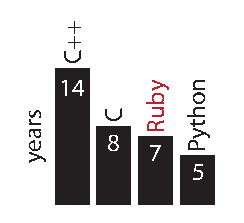
\includegraphics[width=2in]{programming-graph.pdf}%
\vspace{-40pt}%
\end{wrapfigure}%
%
\bigskip
\mhead{Coding \newline Proficiencies}%
\emph{Strong}\ 
\textsc{c},
\Cpp\ (including modern extensions),
Ruby,
Python (including \textsc{c} extensions),
\LaTeX,
shell scripting%,


\medskip
\emph{Familiar}\ 
\textsc{Matlab},
\textsc{Fortran}~95,
Perl,
\textsc{R},
\textsc{sql}

\medskip
\emph{Libraries}\ 
Point Cloud Library$^\dagger$,
\textsc{flann}$^\dagger$ ($k$ nearest neighbors),
\Cpp\ Standard Template Library,
Boost,
\textsc{assimp},
ImageMagick/\Magickpp,
\textsc{atlas},
\textsc{lapack},
\textsc{blas},
\textsc{gnu} Scientific Library,
Open\textsc{gl},
\textsc{glsl},
\textsc{glm},
Eigen,
\textsc{Trick} simulator

\smallskip
$^\dagger${\footnotesize indicates code contributed to library.}

\medskip
\emph{Software}\ 
Git,
Gnuplot,
Emacs,
Vim,
Bash,
Zsh,
\textsc{gcc},
\textsc{gdb},
Valgrind,
\textsc{cm}ake,
Postgre\textsc{sql},
My\textsc{sql},
Ubuntu, Mac \textsc{os\,x}



\bigskip
\mhead{Honors \& \newline Awards}%
White House Champion of Change										\rdate{2014}\newline
National Science Foundation Graduate Research Fellowship			\rdate{2009--2012}\newline
``Best of Austin'' Award: Best Activist	(\emph{The Austin Chronicle})							\rdate{2011}\newline
Scholar, Netroots Nation											\rdate{2011}\newline
Initiate, Friar Society (University of Texas at Austin)				\rdate{2010}\newline
Graduate School Recruitment Fellowship (University of Texas at Austin) \rdate{2007}\newline
Black Belt, Tae Kwon Do (Chung Do Kwan)								\rdate{2006}\newline
Member, Hillcrest Honors Community (Virginia Tech)				\rdate{2003--2007}\newline
Inductee, $\Upsilon\Pi\mathrm{E}$ (Virginia Tech)					\rdate{2006}\newline
Gilbert \& Lucille Seay Scholarship (Virginia Tech)					\rdate{2005}\newline
National Merit Scholarship											\rdate{2002}\newline

\newpage
\mhead{Professional \newline Appointments}%
\textbf{Intuitive Machines,} Houston \newline
\emph{Senior Development Engineer} \rdate{\textsc{jun}~2015--\textsc{present}}
\begin{itemize*}
  \item Responsible for development and maintenance of navigation filter for \textsc{im}'s universal flight software, to be flown on a deorbiter (Terrestrial Return Vehicle, or \textsc{trv}), Moon Express' moon lander, and two drones
  \item Documented and re-derived the entire 27-state filter, including measurement models for \textsc{gps} and star tracker
  \item Wrote and validated sensor models in \textsc{nasa} \textsc{trick} physics simulator
  \item Performed error budget analysis on \textsc{trv}'s navigation system
  \item Developed a relative navigation model for an acoustic ranging-based underground navigation system for a drilling project
\end{itemize*}

\bigskip
\mhead{Academic \newline Appointments}%
\textbf{Applied Space Exploration Laboratory,} West Virginia University \newline
\emph{Post-doctoral Fellow --- Aerospace Engineer} \rdate{\textsc{jan}~2014--\textsc{jun}~2015}
\begin{itemize*}
  \item Developed fast, accurate \textsc{lidar}-based \textsc{6\,dof} pose initialization strategy for non-cooperative rendezvous
  \item Derived/implemented dual inertial state \textsc{mekf} with asynchronous measurement updates, analytically derived bias transition model
  \item Developed open source Open\textsc{gl}-based \textsc{3d} sensor simulator, \textsc{Glidar}
  \item Studied remote sensing technologies for space natural resource surveying and utilization
  \item Collaborated with and mentored grad students and an undergraduate
\end{itemize*}

\medskip
\textbf{Center for Systems \& Synthetic Biology,} The University of Texas at Austin\newline
\emph{National Science Foundation Fellow; Graduate Research Assistant} \rdate{2007--��2014}
\begin{itemize*}
  \item Designed and implemented algorithms and data structures in Python, Perl, Ruby, and \textsc{c}/\Cpp
  \item Formulated hypotheses relating to an aspect of evolutionary theory called deep homology
  \item Wrote software for validating hypotheses, by quickly predicting gene--disease and gene--phenotype associations
  \item Wrote software for automating processing of large sets of proteome data
  \item Researched, designed, and wrote statistical software for searching for genes under various types of selection (positive, purifying, relaxed)
  \item Invalidated a hypothesis about \textsc{hiv} reservoirs using viral evolution simulation
  \item Designed scheme for re-engineering cellular metabolism in \textit{E.~coli}, and partially implemented it (wet lab)
  \item Worked briefly with mass spectrometers (Orbitrap and \textsc{ltq}; wet lab)
\end{itemize*}

\medskip
\textbf{Dept. of Chemistry \& Biochemistry,} The University of Texas at Austin\newline
\emph{Graduate Teaching Assistant} \rdate{2008, 2013}
\begin{itemize*}
  \item Served as \textsc{ta} for Biochemistry, Introduction to Bioinformatics (graduate level), and Chemistry for non-science majors
  \item Rewrote curriculum for Introduction to Bioinformatics in Python (previously in Perl)
\end{itemize*}


\bigskip
\mhead{Community Contributions}

\textbf{Houston CORE: Mask Factory}\newline
\emph{Artist} \rdate{2016}
\begin{itemize*}
  \item Fabricating 1,100 plaster masks to take to Black Rock City in 2016 for visitors to paint under the man
\end{itemize*}

\medskip
\textbf{The Ruby Science Foundation: The SciRuby Project}\newline
\emph{Director \& Co-Founder} \rdate{2012--\textsc{present}}
\begin{itemize*}
  \item Wrote \textsc{Nm}atrix, dense and sparse linear algebra software for Ruby, in \textsc{c}/\Cpp
  \item Organized the SciRuby Project, dedicated to enhancing the Ruby language's numerical and scientific computing facilities
  \item Applied for grants, mentored graduate and undergraduate students
  \item Wrote three successful Google Summer of Code applications and directed mentors
\end{itemize*}

\medskip
\textbf{Austin Swing Syndicate}\newline
\emph{At-Large Board Member} \rdate{2012--2013}\newline
\emph{Secretary} \rdate{2013--2014}
\begin{itemize*}
  \item Revised bylaws, counseled board on non-profit law and best practices
  \item Managed teams of volunteers
  \item Created policy for providing grants to other organizations for events furthering organizational mission of promoting lindy hop, balboa, shag, and other traditional jazz dances
\end{itemize*}

\medskip
\textbf{Texas Gun Sense}\newline
\emph{Founding Board Member} \rdate{2013--2014}\newline
\emph{Advisory Board Member} \rdate{2014--\textsc{present}}
\begin{itemize*}
  \item Co-founded an organization promoting a fact-based dialogue around the belief that gun ownership is an individual right, best preserved by ensuring that firearms stay out of the hands of criminals
  \item Organized and motivated volunteers to testify and lobby at the state level
  \item Wrote bylaws and 501(c)(3) filing (approved on first attempt)
  \item Successfully devised legislative strategies to kill bills, two sessions in a row
  \item Wrote talking points for lawmakers to use in floor debates
  \item Conferred with legislators and Texas Legislative Council to draft a universal background checks bill
  \item Served as official spokesperson, including hundreds of interviews (television, radio, film; list available upon request)
\end{itemize*}


\bigskip
\mhead{Patents}%
\par\vspace{-\baselineskip}Marcotte, E.M.; McGary, K.; Wallingford, J.; Park, T.J.; \textbf{Woods,~J.O.}; Cha,~H.J. 12 August 2012. Orthologous phenotypes and non-obvious human disease models. \textit{U.S.\ Patent Application Publication 2012/0215458 A1}.

\bigskip
\mhead{Articles}%
\par\vspace{-\baselineskip}\textbf{Woods, J.O.}; Christian, J.A. 2016. \textsc{Lidar}-based relative navigation with respect to non-cooperative objects. \textit{Acta Astronautica}.

\medskip
\par\textbf{Woods, J.O.}; Christian, J.A. 2016. \textsc{Glidar}: An OpenGL-based, real-time, and open source 3\textsc{d} sensor simulator for testing computer vision algorithms. \textit{Journal of Imaging 2}(1).

\medskip
\par\textbf{Woods, J.O.}; Tien, M.Z.; Marcotte, E.M. April 2015. Interrogating conserved elements of diseases using Boolean combinations of orthologous phenotypes. \textit{BioR$\chi$iv}.

\medskip
\par\textbf{Woods, J.O.}; Singh-Blom, U.M.; Laurent, J.M.; McGary, K.L.; Marcotte, E.M. January 2013. Prediction of gene--phenotype associations in humans, mice, and plants using phenologs. \textit{BMC Bioinformatics 14}: p. 203.

\medskip
\par Singh-Blom, U.M.; Natarajan, N.; Tewari, A.; \textbf{Woods, J.O.}; Dhillon, I.S.; Marcotte, E.M. January 2013. Prediction and validation of gene--disease associations using methods inspired by social network analyses. \textit{PLoS One 8}(5): e58977.

\medskip
\par McGary, K.L.; Park, T.J.; \textbf{Woods, J.O.}; Cha, H.J.; Wallingford, J.B.; Marcotte, E.M. April 2010. Systematic discovery of nonobvious human disease models through orthologous phenotypes. \textit{Proceedings of the National Academy of Sciences of the United States of America 107}(14): pp. 6544--9.

\medskip
\par Brennan, T.P.; \textbf{Woods, J.O.}; Sedaghat, A.R.; Siliciano, J.D.; Siliciano, R.F.; Wilke, C.O. September 2009. Analysis of human immunodeficiency virus type 1 viremia and provirus in resting $\textsc{cd4}^{+}$ \textsc{t} cells reveals a novel source of residual viremia in patients on antiretroviral therapy. \textit{Journal of Virology 83}(17): pp. 8470--81.

\bigskip
\mhead{Conference \newline Proceedings}%
\par\vspace{-\baselineskip}\textbf{Woods, J.O.}; Christian, J.A.; Evans, T. February 2015. A \textsc{6-dof} pose initialization strategy for \textsc{lidar}-based non-cooperative navigation. In \textit{38th Annual Guidance \& Control Conference}, Breckenridge, CO.

\medskip
Sell, J.L.; Rhodes, A.; \textbf{Woods, J.O.}; Christian, J.A.; Evans, T. 2014. In \textit{AIAA/AAS Astrodynamics Specialist Conference}, San Diego, CA.

\bigskip
\mhead{Posters}%
\par\vspace{-\baselineskip}\textbf{Woods, J.O.}; Singh-Blom, U.M.; Laurent, J.; McGary, K.L.; Marcotte, E.M. 20--25 February 2012. In \textit{Complex Traits: Genomics and Computational Approaches}, Keystone Symposia, Breckenridge, CO.

\medskip
\par \textbf{Woods, J.O.}; Singh-Blom, U.M.; McGary, K.L.; Marcotte, E.M. 13--16 November 2010. In \textit{From Functional Genomics to Systems Biology},  EMBL Heidelberg, Heidelberg, Germany.

\newpage
\mhead{Technical reports}%
\par\vspace{-\baselineskip}\textbf{Woods, J.O.}; Christian, J.A. 17 October 2014. A real-time, software-based \textsc{3d} sensor simulator. ASEL Technical Memorandum: \textit{ASEL--14--005}.

\medskip
\par Sell, J.; Rhodes, A.; \textbf{Woods, J.}; Christian, J.A. 8 May 2014. Theoretical foundations of pose estimation and covariance computation for non-cooperative relative navigation. ASEL Technical Memorandum: \textit{ASEL--14--001}.

\medskip
\par Natarajan, N.; Singh-Blom, U.M.; Tewari, A.; \textbf{Woods, J.O.}; Dhillon, I.S.; Marcotte, E.M. 2011. Predicting gene--disease associations using multiple species data. UTCS Technical Report: \textit{TR--11--37}.


\bigskip
\mhead{Invited Talks}%
\par\vspace{-\baselineskip}\textsc{Sxsw}edu session: Keeping Schools Secure. 11 March 2015.

\medskip
\par Texas Conference on School-Based Law Enforcement: Panel Discussion. 2010.

\bigskip
\mhead{Media \newline appearances}%
\par\vspace{-\baselineskip}\textit{Media appearances available upon request.}

\bigskip
\mhead{Activities \& \newline Interests}%
dance (lindy hop, balboa, flamenco),
circus arts,
weightlifting,
\textsc{mig} welding and metalworking,
carpentry,
chicken husbandry,
beekeeping,
space exploration,
foreign languages

\bigskip
\mhead{Foreign\newline languages}%
English (native tongue)\newline
Spanish (conversational)\newline
Russian (needs refreshing)\newline
%French, German, Mandarin (smattering)

\bigskip
\mhead{References}%
John~Christian\rdate{\href{mailto:john.christian@mail.wvu.edu}{john.christian@mail.wvu.edu}\hskip 0.5cm\href{tel:304-293-3263}{304-293-3263}}\newline
Asst.\ Professor of Aerospace Engineering, West Virginia University

\medskip
Edward~Marcotte\rdate{\href{mailto:marcotte@icmb.utexas.edu}{marcotte@icmb.utexas.edu}\hskip 0.5cm\href{tel:512-471-5435}{512-471-5435}}\newline
Professor of Chemistry \& Biochemistry, The University of Texas at Austin

\medskip
Andy~Ellington\rdate{\href{mailto:ellingtonlab@gmail.com}{ellingtonlab@gmail.com}
\hskip 0.5cm\href{512-471-6445}{512-471-6445}}\newline
Professor of Chemistry \& Biochemistry, The University of Texas at Austin

\medskip
Claus~Wilke\rdate{\href{mailto:wilke@austin.utexas.edu}{wilke@austin.utexas.edu}\hskip 0.5cm\href{512-232-2459}{512-232-2459}}\newline
Chair, Department of Integrative Biology, The University of Texas at Austin


\end{document}